\subsection{Saddle Point Formualtion and Intuition}
Contrary to the typical approach to solving a problem that is in
the minimax formulation, which consists in dualizing
and then solving the resulting convex minimization problem, we keep
the original form. This enables us to consider a richer class
of problems that we can tackle, especially for problems where
dualizing yield a QP that is not efficiently solvable. We first
take a stab at the saddle-point formulation:
\begin{equation}
  \min_{\vec w \in {W}} \max_{\vec z \in {Z}} \sum_i \left( \vec
w^T \vec F_i \vec z_i + \vec c_i^T \vec z_i - \vec w^T \vec f_i(\vec y_i)
\right)
  \label{saddle_point}
\end{equation}

where the $\vec z_i$'s can be identified with the edge and node potentials of a
markov network and satisfy the constraints of the structured problem. The terms
$\vec F_i$ correspond to the matrix with columns $f(\vec x_i, \vec y)$ over labels $\vec y$i.  
The $\vec c_i$'s correspond to the costs of a $\vec z_i$ and can be
identified with the loss $l$ for a label $\vec y_i'$.

In equation \ref{saddle_point}, the term that is opitmized is defined
as:

\begin{equation}
  {L}(\vec w,\vec z) \triangleq \sum_i \vec w^T \vec F_i \vec z_i + \vec
c_i^T - \vec w^T \vec f_i(\vec y_i)
  \label{saddle_obj}
\end{equation}

It is bilinear in $w$ and $z$. We can then imagine two players represented by
$\vec w$ and $\vec z$ that play a zero-sum game. They perform updates using gradients of
the objective w.r.t. their parameters. They then project the result to the set
of feasible points given by the constraints imposed on the structure. We usually
consider Euclidean projections, as there are well-known problems where they are
efficient to compute. However, as seen later, this is not the case for all
problem. This is why Bregman projections will be introduced. Going back to the
zero-sum game, we have the following operator that is used to perform the
updates for both players at the same time.

\begin{equation}
  \begin{pmatrix}
    \begin{array}{c} \nabla_{\vec w} {L}(\vec w,\vec z)\\
      -\nabla_{\vec z_1} {L}(\vec w,\vec z)\\
      \vdots\\
      -\nabla_{\vec z_m} {L}(\vec w,\vec z)
    \end{array}
  \end{pmatrix} =
  \underbrace{
    \begin{pmatrix}
      \begin{array}{cccc}
        0 & \vec F_1 & \dots & \vec F_m\\
        -\vec F_1^T & & &\\
        \vdots & & \vec 0 &\\
        -\vec F_m^T & & &
      \end{array}
    \end{pmatrix}}_{\vec F}
  \underbrace{
    \begin{pmatrix}
      \begin{array}{c}
        \vec w\\
        \vec z_1\\
        \vdots\\
        \vec z_m
      \end{array}
    \end{pmatrix}}_{\vec u}-
  \underbrace{
    \begin{pmatrix}
      \begin{array}{c}
        \sum_i \vec f_i(\vec y_i)\\
        \vec c_1\\
        \vdots\\
        \vec c_m
      \end{array}
    \end{pmatrix}}_{\vec a} = \vec F \vec u - \vec a
  \end{equation}


\clearpage
\subsection{Duality and Gap function}
We can measure the ``goodness'' of the parameters using the gap function
${G}$:
\begin{equation}
  {G}(\vec w, \vec z) \triangleq \left[ \max_{\vec z' \in {Z}}
{L}(\vec w,\vec z') - {L}^* \right] + \left[ {L}^* -
\min_{\vec w' \in {W}} {L}(\vec w', \vec z) \right]
\end{equation}

where ${L}^*$ gives the result of the min-max of the objective
${L}$. When we have a non-optimal point (i.e. not a saddle point), the
gap is strictly positive. At at an optimal point, the gap is exaclty equal to 0.
Now the restricted gap is exactly the same but the min and max are computed over
a set of parameters that are within a certain distance of the start point
$(\hat{\vec u}_{\vec w},\hat{\vec u}_{\vec z}) \in {U}$:
\begin{equation}
  {G}_{D_{\vec w}, D_{\vec z}}(\vec w, \vec z) = \max_{\vec z' \in
{Z}} \left[ {L}(\vec w', \vec z') : d(\vec z, \vec z') \leq
D_{\vec z} \right] - \left [ \min_{\vec w' \in {W}} {L}(\vec w',
\vec z) : d(\vec w, \vec w') \leq D_{\vec w'} \right ]
\end{equation}

The motivation for using this restricted gap function is that if we start
``close'' to an optimal point, of course we will converge more rapidly to it.
This can be seen in the convergence analysis of the method.






We mainly follow the intuition and proofs of
\cite{taskarStructuredPredictionDual2006}.\\
The dual extragradient algorithm from Nesterov gives a convergence guarantee for
the objective ${L}$.\\
We present a simple formulation of the algorithm:
\begin{algorithmic}
  \STATE \textbf{Initialize}: Choose $\hat{\vec u} \in {U}$, set $\vec s^{-1} = 0$.
  \FOR{$t=0$ to $t=\tau$}
  \STATE $\vec v = \mathbf{\Pi}_{{U}}(\hat{\vec u} + \eta \vec s^{t-1})$\\
  \STATE $\vec u^t = \mathbf{\Pi}_{{U}}(\vec v - \eta (\vec F \vec v - \vec a))$\\
  \STATE $\vec s^t =  \vec s^{t-1} - (\vec F \vec u^t - \vec a)$
  \ENDFOR
  \RETURN $\overline{\vec u^{\tau}} = \frac{1}{1 + \tau} \sum_{t=0}^{\tau} \vec u^t$
\end{algorithmic}

This algorithm has a lookahead step (i.e. $v$) that serves the peform the actual
gradient update $u^t$. The intuition behind the lookahead step is that given a
function to optimize that is Lipschitz, Nesterov was able to show that we can
upper bound $f_{D}(\bar{u}^n) = \max_y \left \{ \langle g(y),\bar{u}^n - y
\rangle : d(\hat{u},y) \leq D \right \}$, where $\bar{u}^n is the weighted
average over all the updates $u^t$ up to iteration n. The function g corresponds
to the objective ${L}$ in our setting. When value of $f_D(\bar{u}^n)$
gets close to 0, we have that the value $g(y^*)$ for an optimal $y^*$ is close
to 0, which signifies that we have reached saddle point (i.e. what we wanted).
Note that in the definition of $f_D$, we used a
distance metric d. This corresponds to the Euclidean distance (or Bregman
distance in non-Euclidean setting). The rojection operator $\Pi_{{U}}$
in the algorithm simply projects a point back to the set ${U}$ by
finding the nearest point with respect to the distance metric used.

\clearpage
\subsubsection{Non-Euclidean setting}
The main problem with the Euclidean projection operator is that for many
problems, it is hard to compute the projection. Indeed for min-cut, we need to
compute the partition function first, which is \#P-complete. Thus, the authors
of the paper introduced the Bregman operator, which computes the projection
using the Bregmand divergence. Using this operator has the great advantage of
being easier to compute. We can see this for $L1$ regularization. Computing a
projection using $L1$ distance is hard since it is not differentiable. Using the
negative entropy as our function h (see \ref{proxstep}), we get that the Bregman divergence is the KL divergence. This
implies that we can differentiate the divergence to get the parameter that
minimizes it. It is worth mentioning that for some problems, projections can
still be hard to compute. This is why it may be wise to move to the FW algorithm
especially if solving a linear problem over constraints the constraints is easy (or ``easier'').

\subsubsection{Memory-efficient tweak}
In the dual extragradient algorithm, both a vector $s^t$ and a vector
$\bar{u}^t$ are maintained. However, we can observe that the $s_t$'s can be
found using the running average $\bar{u^t}$ since $s^t = -(t + 1 ) \sum_{i=0}^t
(F \bar{u}^t - a)$. We only have to store the vector $\bar{u}^t$. We can even do
better when $|{Z}| \gg |{W}|$ since $\bar{u}^t = \{
\bar{u}_w^t,\bar{u}_z^t \}$ and we only care about the part that corresponds to
$w$. $\bar{u}_z^t$ is maintained implicitly by storing a vector of size
$|{W}|$ (although we now need to store $s_w^t$). It can be reconstructed
using $\bar{u}_w^t$.
% The following figure:
% illustrates the various dependencies.
\begin{figure}
  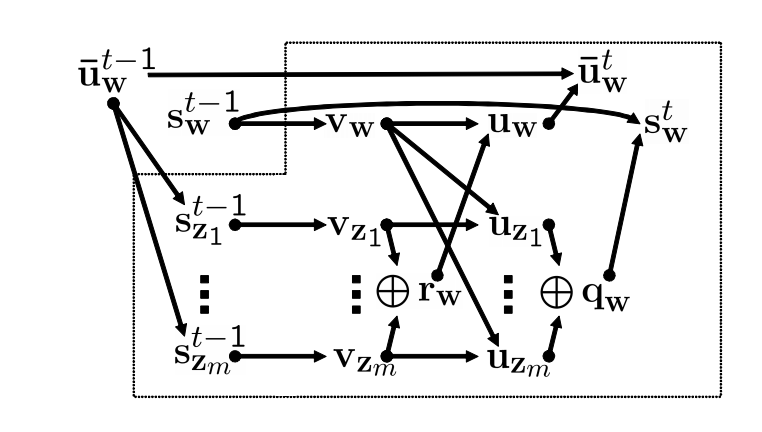
\includegraphics{figures/mem_tweak.png}
  \label{memtweak}
  \caption{Memory efficient algorithm}

%%% Local Variables:
%%% mode: latex
%%% TeX-master: "mainProject"
%%% End:
